\begin{figure}[htbp]
\centering
\caption[A priori ANC and Nitrate Power Graph]{A priori ANC and Nitrate Power Graph.  The power graphs for ANC and Nitrate are the same because they both have the same number of predictors.}
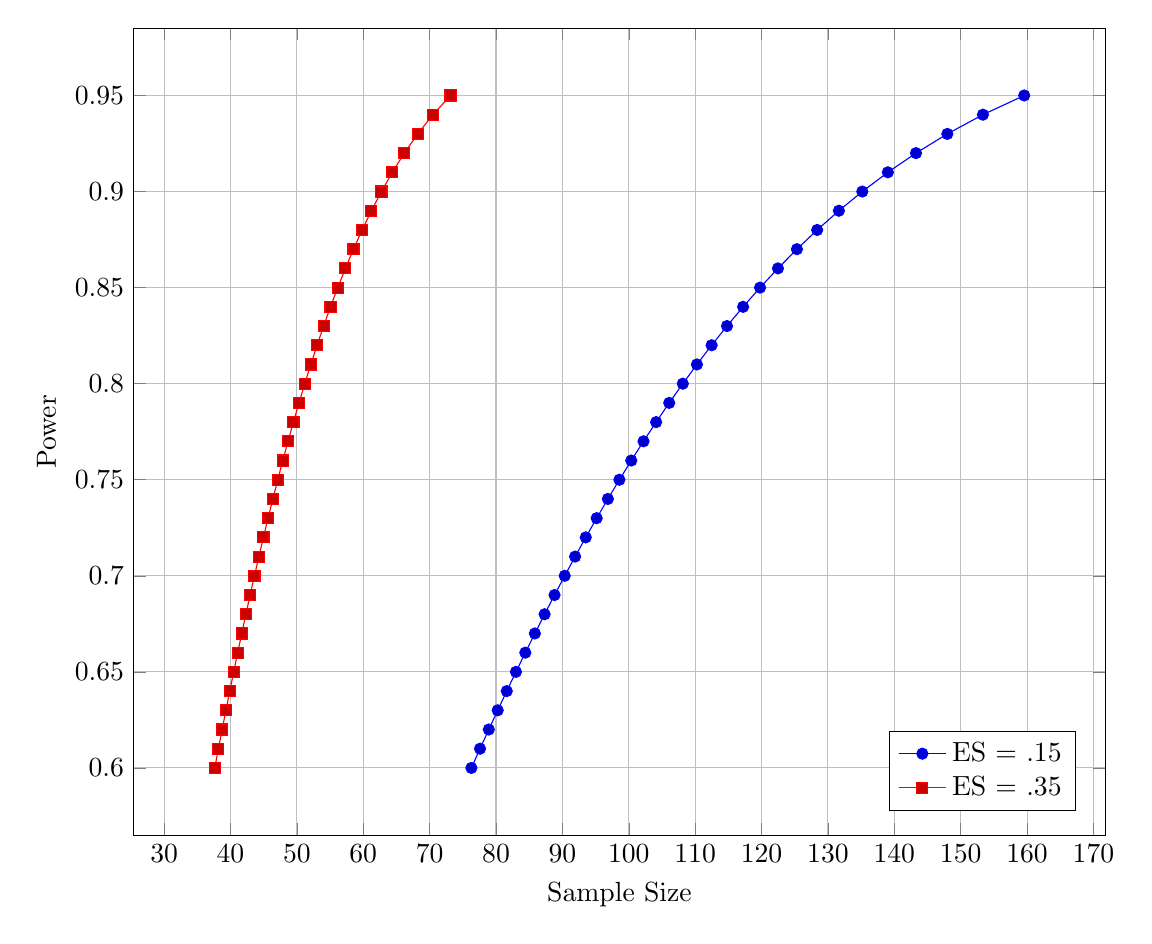
\begin{tikzpicture}
	\begin{axis}[grid=major,xlabel=Sample Size,ylabel=Power,scale=1.8, legend pos= south east] 
\addplot coordinates{
(76.2911	,0.60)
(77.592,	0.61)
(78.9124,	0.62)
(80.2534	,0.63)
(81.6164	,0.64)
(83.0029	,0.65)
(84.4146,	0.66)
(85.853	,0.67)
(87.32,	0.68)
(88.8177,	0.69)
(90.3482,	0.70)
(91.914,	0.71)
(93.5176,	0.72)
(95.162,	0.73)
(96.8504	,0.74)
(98.5864,	0.75)
(100.374,	0.76)
(102.218,	0.77)
(104.122,	0.78)
(106.094,0.79)
(108.139,	0.80)
(110.265,	0.81)
(112.48,	0.82)
(114.795,	0.83)
(117.222,	0.84)
(119.775	,0.85)
(122.471,	0.86)
(125.33,	0.87)
(128.378,	0.88)
(131.647,	0.89)
(135.179,	0.90)
(139.027,	0.91)
(143.263,	0.92)
(147.987,	0.93)
(153.347,	0.94)
(159.566,	0.95)};
\addlegendentry{ES = .15}

\addplot coordinates{
(37.6275,	0.60)
(38.1808,	0.61)
(38.7424,	0.62)
(39.3129,	0.63)
(39.8929,	0.64)
(40.4829,	0.65)
(41.0838,	0.66)
(41.6961,	0.67)
(42.3208,	0.68)
(42.9585,	0.69)
(43.6104,	0.70)
(44.2774,	0.71)
(44.9606,	0.72)
(45.6612,	0.73)
(46.3808,	0.74)
(47.1207,	0.75)
(47.8827,	0.76)
(48.6687,	0.77)
(49.4809,	0.78)
(50.3216,	0.79)
(51.1938,	0.80)
(52.1007,	0.81)
(53.0458,	0.82)
(54.0337,	0.83)
(55.0693,	0.84)
(56.1588,	0.85)
(57.3093,	0.86)
(58.5299,	0.87)
(59.8314,	0.88)
(61.2275	,0.89)
(62.7358,	0.90)
(64.3793,	0.91)
(66.1888,	0.92)
(68.2074,	0.93)
(70.4977,	0.94)
(73.1559,	0.95)};
\addlegendentry{ES = .35}

				
\end{axis}
\end{tikzpicture}
\label{fig:ANCnNPowerGraph}
\end{figure}